Will follow an in depth analysis of each threat previously mentioned in the threat model after a breaf explanation of the security properties of our system.
Each subsection will explain for each threat the scenario and its causes, providing also the consequent residual risk.

\begin{table}[H]
    \centering
    \begin{tabular}[c]{|>{\raggedright\arraybackslash}m{0.3\textwidth}|>{\raggedright\arraybackslash}m{0.3\textwidth}|>{\raggedright\arraybackslash}m{0.3\textwidth}|}
        \hline
        \textit{\textbf{Threat}} & \textit{\textbf{Attack Goal}}       & \textit{\textbf{PABEL Mitigation}}   \\ \hline
        Unauthorized user        & Read protected data                 & Human authentication + ABE           \\ \hline
        Unauthorized agent       & Read protected data                 & Agent identity + ABE                 \\ \hline
        User-Agent Collusion     & Bypass policy                       & Combined attributes                  \\ \hline
        Prompt injection         & Trick agent into requesting secrets & Interception + authorization         \\ \hline
        Agent Impersonation      & Fake agent identity                 & Installation credentials             \\ \hline
        Credential theft         & Obtain a secret to act as a user or an installation & Both principals required, revocable credentials \\ \hline
        Network attacker         & Steal / forge traffic               & \raggedright Token verification + TLS {[}+ VPN{]} (see Section \ref{Future Development})\arraybackslash \\ \hline
        Compromised endpoint     & Read plaintext                      & Out of scope                         \\ \hline
        Master Key compromise    & Decrypt everything                  & Operational key protection           \\ \hline
        Post-decryption leakage  & Exfiltrate plaintext                & Out of scope / limitation            \\ \hline
    \end{tabular}
    \caption{Summary of various possible threat scenarios}
\end{table}

\subsection{Security Properties}
It is important to note, that the analysis refers to five properties of the system:
\begin{enumerate}
  \item[\textbf{P1}] \textbf{Two authentication, on every call.} The human and the agent are verified on every request; nothing is kept as ``logged in''.
  \item[\textbf{P2}] \textbf{Cryptographic, per-section enforcement.} A section opens only if the combined key satisfies its policy; the server does not filter, it is unable to open the others.
  \item[\textbf{P3}] \textbf{No key or credential at the agent.} Keys stay on the server and, for harnesses with a hook, the credentials of the installation are injected by the hook and are not readable by the model.
  \item[\textbf{P4}] \textbf{Accountability.} Every call that reaches the server leaves a record with user, agent and outcome.
  \item[\textbf{P5}] \textbf{Fail-closed interception.} Once the hook runs and there is an authentication or relay's error, it all ends in a denial and never in a direct read.
\end{enumerate}

\subsection{Unauthorized User}
The attacker is a person who holds no attribute that satisfies the policy of a section; it can be an employee outside the required department or even an outsider with a stolen password.
They could try to obtain a token without the 2FA, but the only way to login is the Authorization Code flow that is hosted by the identity provider and PABEL's client doesn't enable direct password grant, so any attempt without the 2FA authorized by the realm is uneffective.

An attacker could also attempt to raise its own attributes, but those fed a key that can only be edited by an administrator, never by a user.
Even a forged token wouldn't work, since the server verifies its signature against the keys published by the realm and also its issuer and expiration.

Finaly, a malevolent actor could try to directly read the file, but everything sensible is in form of a ciphertext, hence the cryptography is the security measure.
No key without the correct attributes satisfies a given policy, thus cannot decrypt it \cite{bethencourt2007ciphertext}: the denial does not rest on a check that could be skipped.

\paragraph{Residual risk} A user is, by design, able to read what their attributes allow and what they do with it is addressed in section \ref{sec:postdecryption}.

\subsection{Unauthorized Agent}
The attacker is an agent that the organization has not approved, or an apporved one that must not serve a given user.
An installation that is unknown, revoked or belonging to a disabled product will always fail the verification and the request will be denied.
In case of a valid installation, but used by someone not intended or simply wihtout the role required by its product is not rejected, but instead is treate like it has no attributes, thus every section which name the agent will stay close.

\paragraph{Residual risk} The consequences of this design must be kept in mind by who writes the policies.
A section whose policy does not name any agent is satisfied by the user alone through \textit{any} recognized installation.
Restricting a section to some agents is done by naming them in its policy and restricting \textit{any} agent by defining an unobtainable attribute (e.g. say "\code{no-agent}" that will not be addressed to any agent, see section \ref{CPvsKP}).

\subsection{User-Agent Collusion}
In this scenario the attacker is a user who handles an agent, possibly one under their control, and tries to obtain together more than each of them is entitled to.
The key used in a request is built for one pair and it carries exactly the union of the attributes of both user and installation in use. A section whose policy requires both, such as \code{sales and agent\_claude\_code}, opens for that pair and this is the intended meaning of the policy rather than a leak.
The structure itself is anti-collusion, i.e. nothing in the pair can add attributes that neither holds.

It is important to underline that even a user with two installations cannot merge them, since a request uses only one of them and having one with two agents would never be satisfied.

\subsection{Prompt Injection}
Content processed by the agent (a page, a file, the output of a tool, etc...) carries instruction that do not correspont to the ones of the user (e.g. read a protected document, obtain credential, disable enforcement, etc...).

An attacker could controls the content but nothing else, neither the machine nor the tokens.
They could ask ultimately three things:
\begin{enumerate}
    \item An attacker could ask for a document the user cannot read: this fails since the key is determined by the authenticated identities of user and installation, not by anything written in a prompt;
    \item It could be ask to obtain credential or to disable the enforcement, but here the hook denies the request and it is not part of the reasoning of the model, hence it decides on the shape of the call (see Table \ref{tab:decide});
    \item Lastly, an injection could try to read something that the user is entitled to read, but any mechanism of the system prevents that (see Section \ref{sec:postdecryption}).
\end{enumerate}
\paragraph{Residual risk} For agents without hooks the second scenario is not blocked and the risk actually resides in the fact that installations are not shielded from the model (Section \ref{Two Classes of Agents}), still keeping the security assurances given by the cryptography, since protected files remain ciphertext.

\subsection{Agent Impersonation}\label{sec:impersonation}
A compromised or manipulated agent tries to act as another installation, to obtain the attributes of a more privileged harness.
The identity of the agent is the verified \code{azp} claim of a token that Keycloak issued, never a value the caller declares (Section \ref{Agent Identity Model}).
On the "hooked client", the hook denies the two routes that would let the model choose an identity, that is rewriting the configuration (\code{DENY\_CONFIG\_TAMPER}) or invoking the functionalities directly with a chosen agent (\code{DENY\_HOOK\_BYPASS}).

The second denial was added after a live session of GitHub Copilot. It was observed that it was calling the relay from a shell command with the identifier of another harness, to "borrow" its credential.
\paragraph{Residual risk} The credential of an installation is stored in a directory of the client machine. For harnesses with hooks the model cannot read it, for MCP-only harnesses this protection does not exist. A stolen credential could be revoked by flagging as such said installation.

\subsection{Credential Theft}
The objects worth stealing are three: human's session, installation's secret and the keys cached in the database.
Any of these, singularly taken, is not enough to read a protected document.
An attacker, with only a user token could obtain a key that lacks the attributes of the agent, thus every section tied to a specific agent stays closed; vice versa if an attacker has only an installation token it will still require a human login with 2FA.
In any case tokens have a limited lifetime, furthermore, an installation can be revoked simply fagging it and a user could be easily disabled by the identity provider.

\paragraph{Residual risk} The cached keys are decryption keys: whoever holds them can decrypt offline whatever attributes they satisfy, althoudh they cannot generate other keys.
\textbf{N.B.} In this work, both keys and secrets are, respectively, in PostgreSQL and in a directory of the client, with no further protection (see Section \ref{Future Development}).

\subsection{Network Attacker}
An attacker observes or modifies the traffic between client and server.
Forging a request does not work because a token whose signature, issuer and expiration do not check is rejected.
Even intercepting the authorization code in the redirect towards the local machine is of no use without the verifier, which is never sent with the code \cite{rfc7636}.

\paragraph{Residual risk} The response of the server carries the plaintext of each section the pair may read and a bearer token can be replayed by whoever observes it during its validity.
Those issues can be mitigated via encryption and confining the system inside a VPN (see Section \ref{Future Development}).

\subsection{Compromised Endpoint}
An attacker who controls the client machine, act with the privileges of its user, so he can remove or bypass the hook and read the credentials stored there.
This scenario, however, is declared out of scope in the adversary model (Section \ref{Motivation and Threat Model}).
The consequences are nevertheless bounded, since document not yet read are still ciphertext and the server applies the same checks to every call, thus the attacker gets at most what the stolen identities allow.

\subsection{Master Key Compromise}
Whoever holds the master secret key can generate a key for any set of attributes and no policy could resist them: the authority is the root of trust of the whole system (Section \ref{Background}).
Ideally, the key is created inside the server, never sent elsewhere and used only by the server itself whithin the scope of the authoring tool (see \nameref{ABEditor}).
Its custody is assumed in the threat model (Section \ref{Motivation and Threat Model}) and the only remedy to such scenario is a new authority that would make previous encrypted document unreadable.

\subsection{Post-Decryption Leakage}\label{sec:postdecryption}
When the server outputs the decrypted data to the agent, the guarantees of PABEL end (as shown in Figure \ref{fig:boundary}).
The agent, its vendor, the user or an injected instruction can send them anywhere and no application-level mechanism can prevent it.
What the system offers is minimization and accountability: only the sections that the user and the agent are entitled to are released, not the whole document; every release is recorded with the number of readable sections and the copies explicitly requested are deleted at the end of the session via session-end hook.
\begin{figure}[H]
    \centering
    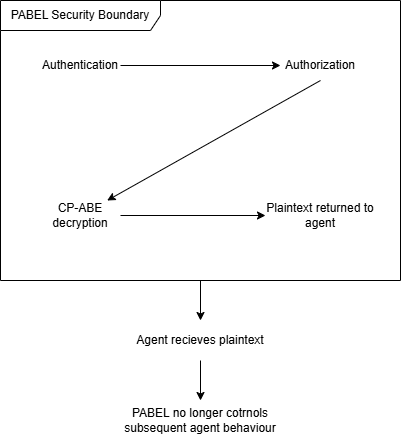
\includegraphics[width=0.8\textwidth]{media/diagrams/Security Boundary.png}
    \caption{PABEL's security boundary}\label{fig:boundary}
\end{figure}
\paragraph{Residual risk} The data exposed to the vendor is exactly the data the policy allows and no more; what the vendor, the model or the user does with it is outside the control of this work.

\subsection{Limitations}
Several limitations of this work, notably the unencrypted transport, the protection of keys and secrets at rest and the verification of the audience of the tokens, are listed in Table~\ref{tab:target} together with the deployment they are expected to reach (Section~\ref{Future Development}).
Other limitations that belong to the design are:
\begin{itemize}
  \item The interception is as strong as the hook: a user can theoretically remove it, a harness without hooks is not enforced and where the wiring is missing the read is not intercepted, although the file remains ciphertext.
  \item The local log of the connector records the outcomes for a third party who later obtains it, but it cannot protect against the agent it records; the trail of the server is the record, and it covers only the calls that reach the server.
  \item A single authority holds the master key and replacing it invalidates every existing document.
  \item Only the harness is identified, never the model and the enforcement operates at the application level.
  \item A policy that does not name an agent is satisfied by any recognised installation.
\end{itemize}
